
\documentclass{standalone}
\usepackage{graphicx} % Required for inserting images
\usepackage{tikz}
\usepackage{pgfplots}
\usepgfplotslibrary{colorbrewer} % LATEX and plain TEX
\usepgfplotslibrary[colorbrewer] % ConTEXt
\usetikzlibrary{pgfplots.colorbrewer} % LATEX and plain TEX
\usetikzlibrary[pgfplots.colorbrewer] % ConTEXt
\usepgfplotslibrary{groupplots}

\begin{document}
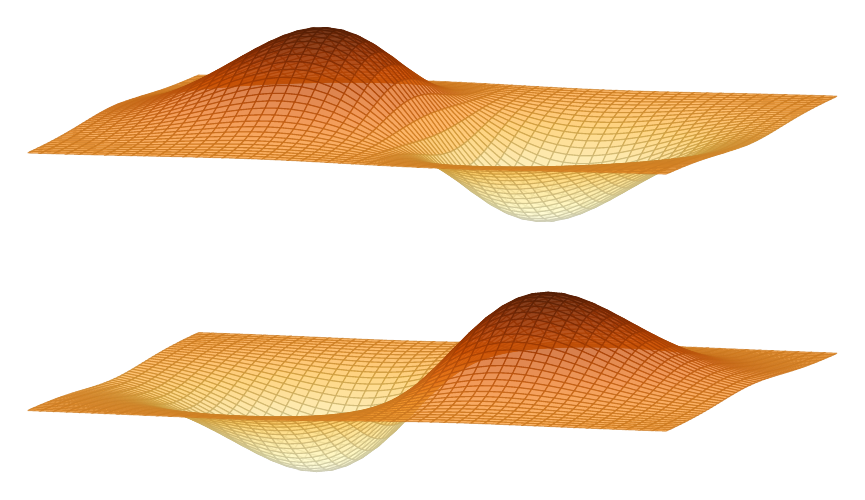
\begin{tikzpicture}
    \begin{groupplot}[
        group style={
            group size=1 by 2, % 1 column, 3 rows
            vertical sep=-150pt % No space between plots
        },
        xlabel={$x$},
        ylabel={$y$},
        zlabel={$z$},
        zmin=-2, zmax=2,
        colormap/YlOrBr,
        view={15}{8},
        scale=1.5,
        hide axis
    ]
    
    \nextgroupplot
    \addplot3[
        surf,
        %shader=faceted interp, % Combines facets with smooth shading
        opacity=0.7, % Adjust opacity as needed
        domain=-2:2,
        domain y=-2:2,
        samples=50 % Increase samples for a smoother appearance
    ]
    {-1.5*x/e^(x^2 + y^2)};

    \nextgroupplot
    \addplot3[
        surf,
        %shader=faceted interp, % Combines facets with smooth shading
        opacity=0.7, % Adjust opacity as needed
        domain=-2:2,
        domain y=-2:2,
        samples=50 % Increase samples for a smoother appearance
    ]
    {1.5*x/e^(x^2 + y^2)};
    
    \end{groupplot}
    \end{tikzpicture}


\end{document}